% !TEX encoding = UTF-8
% !TEX TS-program = pdflatex
% !TEX root = ../tesi.tex
% !TEX spellcheck = it-IT

%**************************************************************
\chapter{Project Development}
\label{cap:project-development}
%**************************************************************

\intro{In this chapter describes the solved tasks of the project}\\

%**************************************************************
\section{SAM file creation}
First, to procede with the project, I've created the SAM file by using the \emph{Burrows-Wheeler Aligner} supplied by BWA.
The software can be found here: \href{http://bio-bwa.sourceforge.net}{http://bio-bwa.sourceforge.net}

The first typed command, necessary for the file creation is:
\\
\\
\verb|bwa index Lactobacillus_casei_genome.fasta|
\\
\\
This command allows to index the fasta genome file. The indexing of the genome's file allows the increasing of the performance during the genome alignment phase.\\

The second typed command is:
\\
\\
\verb|bwa -t 4 mem Lactobacillus_casei_genome.fasta lact_sp.read1.fastq lact_sp.read2.fastq > Lactobacillus_casei_genome.sam|
\\
\\
This command allows the alignment of the two reads files on the reference genome file into a SAM file that serves for the project.\\

There are others different instruments that allows this, but BWA should be the best tools especially for the performances.\\

The goal file contains all the information about the resequenced genome in according with the SAM specifications.
The weight of the file is more or less around 890MB.
\newpage

\section{Insertion length}
For this task I wrote an algorithm, that, for each row of the SAM file (which contains information about the resequencing), extracts the values obtained from :
\\
\\
\verb|abs(POS - PNEXT)|
\\
\\
\emph{POS} is the start of the read and \emph{PNEXT} is the start position of the next read.\\
For the research of the insert size length, there are some different opinions that come from different sources, some of these suggest to use only the \emph{TLEN} field of the SAM file to calculate the insert size length.
\\\\
Once I've extracted all the insertion length, I plot all the data in a barchart track, as you can see here \ref{fig:1}.\\
This track allows to identify the wrong lectures and the wrong reads.
\\\\
For this track, a R script was made; from this chart, as I've already written, it's possible to analize the reads that have the wrong insert values, which in some cases, is over 2 million bases long.\\

This error can be partially explained by the multiple alignment of the reads on reference genome.
\newpage
 \begin{figure}[H]
				\centering
				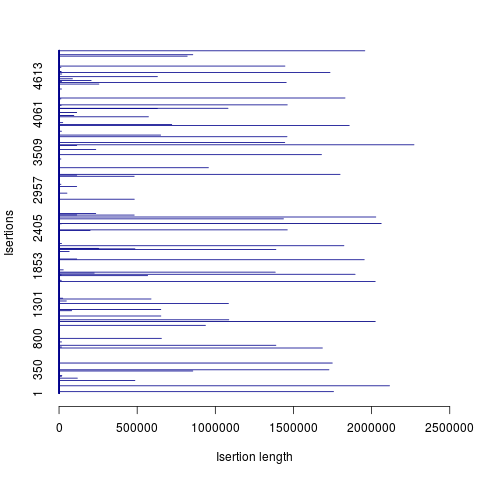
\includegraphics[scale=0.8]{immagini/r.png}
				\caption{Barchart for the isize without exluding errors, the chart includes only the first 10.000 reads}\label{fig:1}
				\end{figure}

From this track, it's possibile to see how some reads that have the insert lenght longer than 10.000 bases, have an error, so according to the mean and the standard deviation, these reads are to be excluded.
Here \ref{fig:2} you can see the track that exludes the reads with insert equal to or greater thn 10.000 bases long. The obtained chart is more correct than the first chart.
 \begin{figure}[H]
				\centering
				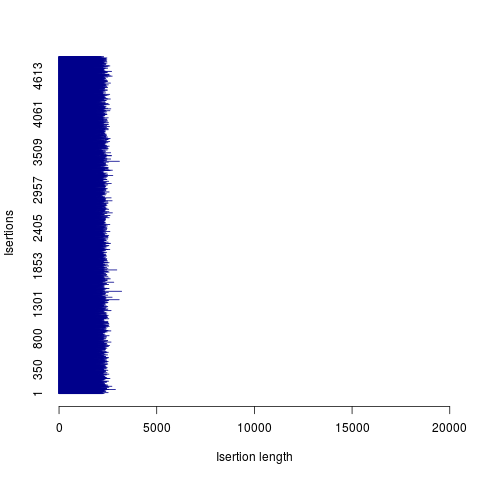
\includegraphics[scale=0.8]{immagini/r1.png}
				\caption{Barchart for the isize without errors}\label{fig:2}
				\end{figure}

The result of the mean and standard deviation are:
\begin{itemize}
\item \begin{description}
		\item[MEAN:] 2102
  \end{description}
\end{itemize}

\begin{itemize}
\item \begin{description}
		\item[STD:] 236.85
  \end{description}
\end{itemize}


The result of this task, also, can be found inside a csv file, that allows to create a barchart with the insertions size obtained by the R script.

\section{Physical Coverage}

The Physical Coverage is calculated by an algorithm really similar to the given Perl script.\\

The main reason is the optimization of the algorithm.\\\\

The algorithm, infact, loops on half of the reads by checking if the \emph{TLEN} is greater than 0.\\
At first, I created an array where each cell was intialized to 0. 
In each one of these cells, I put +1 when the index is equal to the read start position, and I put -1 when the index is equal to the next read start position.\\

It's necessary to mention that the used reads, are only the right aligned reads, and the filtering of the right-wrong reads is made by checking the \emph{FLAG} field of the SAM file.
\\
The resultant values are put inside a wig file, called \emph{physical\_coverage.wig}.

After that, the file was loaded onto IGV to show the physical coverage, in order to start making hypotesys and analisys about some structural variations.

Some small part of resultant tracks produced by the IGV are reported below:

 \begin{figure}[H]
				\centering
				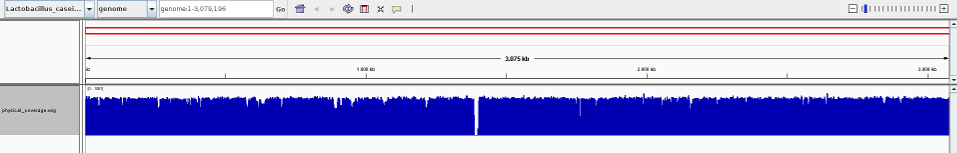
\includegraphics[scale=0.6]{immagini/physical_coverage_1.png}
				\caption{Whole sequence coverage}\label{fig:6}
				\end{figure}


 \begin{figure}[H]
				\centering
				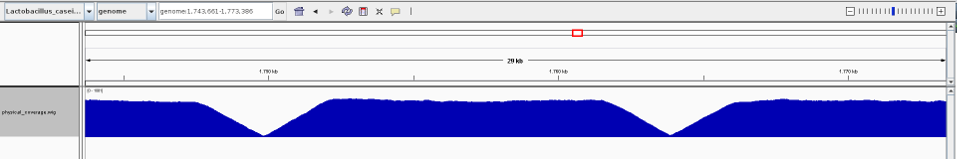
\includegraphics[scale=0.6]{immagini/physical_coverage_2.png}
				\caption{Sequence coverage, in the same position of the physiscal coverage, identifies an inversion structural modification}\label{fig:7}
				\end{figure}
				
				
				
 \begin{figure}[H]
				\centering
				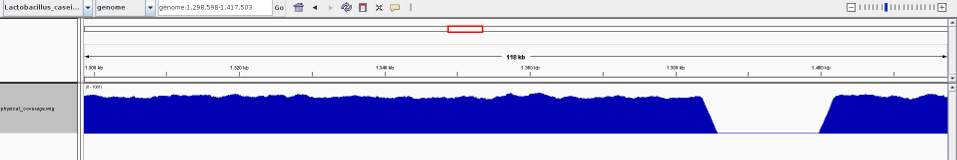
\includegraphics[scale=0.6]{immagini/physical_coverage_3.png}
				\caption{Sequence coverage that identifies an structural variation, in particular, a long deletation}\label{fig:8}
				\end{figure}				


\section{Sequence Coverage}
The Sequence Coverage is calulated by the algorithm contained inside the SequenceCoverageAlgorithm.py.\\
This algorithm is similar to the physical coverage script's, but, with the difference that it is necessary for the read to have the positive and the negative \emph{TLEN} value.\\
As well the Physical coverage, also, this algorithm make a check on the \emph{FLAG} field
\\
\\

At first, I created an array in which each cell is intialized to 0.
Then for each cell that has the index between START and START + sequence lenght, I put +1.
This step is necessary for each compatible reads.\\\\

The resultant values are put inside a wig file, called \emph{sequeence\_coverage.wig}.

After that, the file is loaded onto IGV to show the sequence coverage to help making hypotesys and analisys about some structural variations.

Some small part of resultant tracks produced by the IGV are reported below:


 \begin{figure}[H]
				\centering
				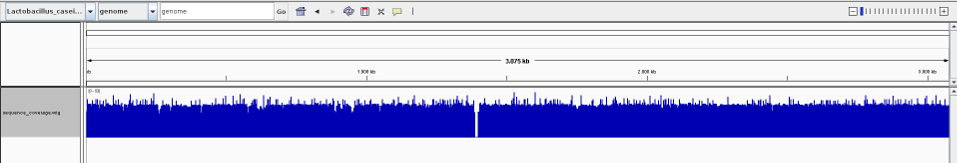
\includegraphics[scale=0.6]{immagini/sequence_coverage_1.png}
				\caption{Whole physical coverage}\label{fig:9}
				\end{figure}


 \begin{figure}[H]
				\centering
				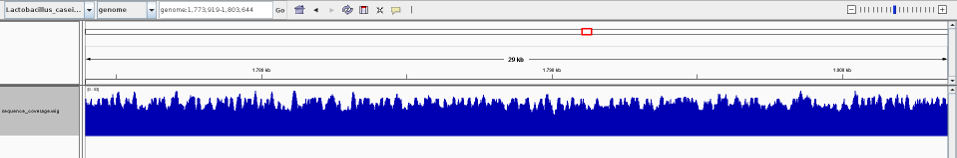
\includegraphics[scale=0.6]{immagini/sequence_coverage_2.png}
				\caption{Physical coverage that identifies an structural variation}\label{fig:10}
				\end{figure}
				
				
				
 \begin{figure}[H]
				\centering
				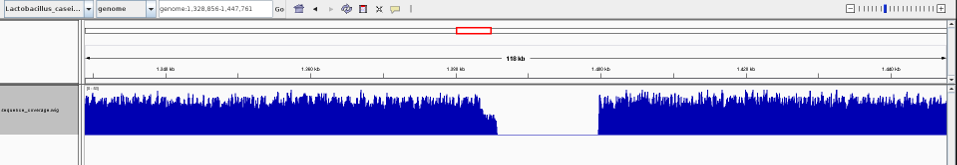
\includegraphics[scale=0.6]{immagini/sequence_coverage_3.png}
				\caption{Physical coverage that identifies a structural variation}\label{fig:11}
				\end{figure}	
				
				

\section{Cigar H and S reads}
\label{sec:cigar}
This algorithm allows to find and map the bases that are in the clipped reads.\\
As written in SAM file specifications, there are two kinds of clipping:

\begin{itemize}
\item \begin{description}
		\item[S:] soft clipping (clipped sequences present in SEQ)
  \end{description}
\end{itemize}

\begin{itemize}
\item \begin{description}
		\item[H:] hard clipping (clipped sequences NOT present in SEQ)
  \end{description}
\end{itemize}


This algorithm tracks the coverage of the reads with the hard-soft clipping. Below is reported the whole track of this.
 \begin{figure}[H]
				\centering
				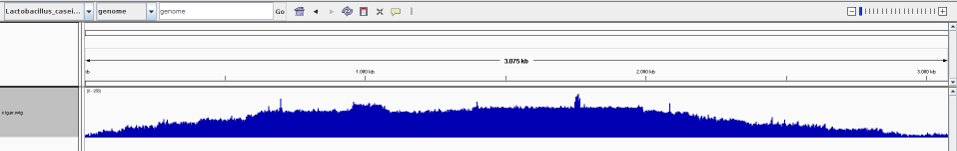
\includegraphics[scale=0.45]{immagini/cigar_coverage_1.png}
				\caption{Whole coverage of the bases involved in a clipping}\label{fig:15}
				\end{figure}	
				
It's interesting to see how in corresponding postion of the structural inversions, the cigar's track has some peaks:

 \begin{figure}[H]
				\centering
				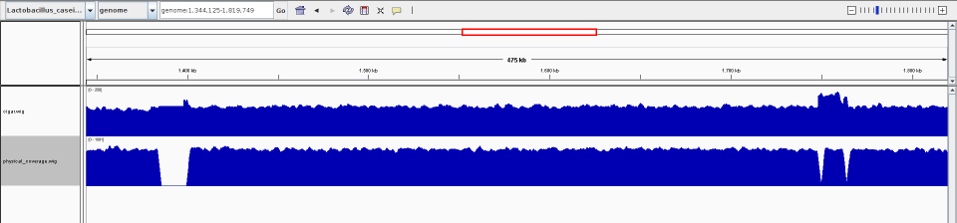
\includegraphics[scale=0.45]{immagini/cigar_coverage_2.png}
				\caption{Cigar coverage and physical coverage that allow to undestand the structural varations}\label{fig:16}
				\end{figure}	
As we can see in the figure \ref{fig:16}, in the proximity of the deletetation and especially in proximity of the inversion structural variations, the cigar's track has peaks; these peaks allow to understand and to confirm the presence of the strutural variations.		

						
\section{Kmers counting}
To start talking about the kmers, it is necessay to define what it is.
\begin{quote}
The term k-mer typically refers to all the possible substrings of length k that are contained in a string. In computational genomics, k-mers refer to all the possible subsequences (of length k) from a read obtained through DNA Sequencing
\end{quote}

The algorithm for the kmers analisys is inside the KmersAlgorithm.py.\\
In order to work, the algorithm expects the kmers length value, many different tests were made using 7-mers, 4-mers and 9-mers.\\
The result is really different and to make some hypotesys or analisys it is necessary to plot different barchart by usign some R scripts.\\\\

These tracks have allowed us to learn and see what are the most, and the less present kmers inside the resequenced genome.\\

The algorithm considerz each kmers with the relative opposite, the goal is to eliminate the errors that could comes from the "string slicing" from the kmers build.\\\\

The algorithm starts from position 0 of each \emph{SEQ} and terminate with the end of \emph{SEQ}.
In each loop made on the SEQ string, the algorithm moves the start position from \verb|i| to \verb|i+1| and the end position from \verb|end| to \verb|end+1|.\\
The resultant substring is exactly as long as we expected.\\\\

I reported the tracks generated by the different k dimensions below:

 \begin{figure}[H]
				\centering
				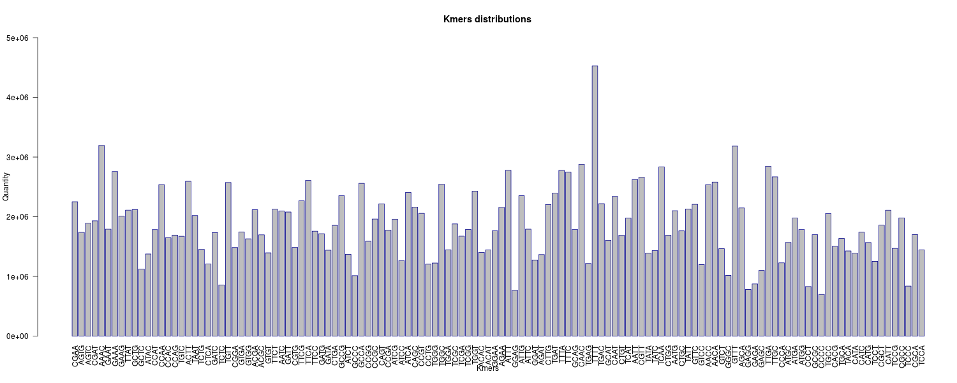
\includegraphics[scale=0.45]{immagini/kmers_4.png}
				\caption{Kmers with k = 4}\label{fig:12}
				\end{figure}


 \begin{figure}[H]
				\centering
				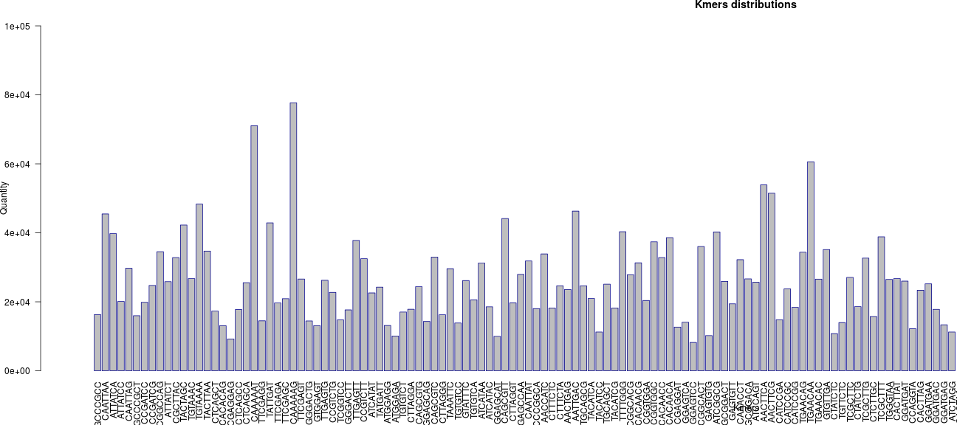
\includegraphics[scale=0.45]{immagini/kmers_7.png}
				\caption{Kmers with k = 7}\label{fig:13}
				\end{figure}
				
				
				
 \begin{figure}[H]
				\centering
				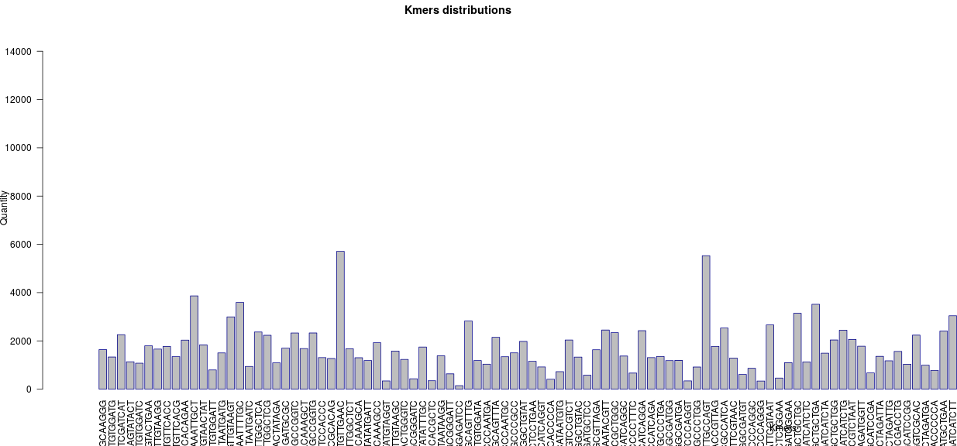
\includegraphics[scale=0.45]{immagini/kmers_9.png}
				\caption{Kmers with k = 9}\label{fig:14}
				\end{figure}	
				
In these tracks it's simple to see what kmers are more frequent than others, the observation of the kmers and the relative bases is helpful for the gene recongition, because it allows the reasearch of a certain protein.\\\\
The result of this algorithm is a csv file that maps kmer name with the kmer frequence				
